\documentclass{llncs}
\input{glyphtounicode}
\pdfgentounicode=1
\usepackage{graphicx,booktabs,tabularx,amsmath,amssymb}
\usepackage{accsupp}
\usepackage[hidelinks]{hyperref}
\hypersetup{pdfauthor={},pdftitle={Graph Representations for Congestion Onset Prediction: A Controlled Comparative Study}}
\newcommand{\TestOnAG}{0.01602}
\newcommand{\TestAllAG}{0.02060}
\newcommand{\TestCalOnAG}{0.01397}
\newcommand{\TestCalAllAG}{0.01874}
\newcommand{\TestRecallAG}{93.46\%}
\newcommand{\TestFprAG}{4.87\%}
\newcommand{\TestOnRUnion}{0.01425}
\newcommand{\TestAllRUnion}{0.01852}
\newcommand{\TestCalOnRUnion}{0.01286}
\newcommand{\TestCalAllRUnion}{0.01712}
\newcommand{\TestRecallRUnion}{96.15\%}
\newcommand{\TestFprRUnion}{5.29\%}
\newcommand{\TestOnAMono}{0.01467}
\newcommand{\TestAllAMono}{0.01920}
\newcommand{\TestCalOnAMono}{0.01381}
\newcommand{\TestCalAllAMono}{0.01870}
\newcommand{\TestRecallAMono}{93.46\%}
\newcommand{\TestFprAMono}{4.87\%}
\newcommand{\TestOnB}{0.01521}
\newcommand{\TestAllB}{0.01974}
\newcommand{\TestCalOnB}{0.01399}
\newcommand{\TestCalAllB}{0.01923}
\newcommand{\TestRecallB}{92.82\%}
\newcommand{\TestFprB}{5.97\%}
\newcommand{\TestOnK}{0.01535}
\newcommand{\TestAllK}{0.01993}
\newcommand{\TestCalOnK}{0.01412}
\newcommand{\TestCalAllK}{0.01960}
\newcommand{\TestRecallK}{93.21\%}
\newcommand{\TestFprK}{5.84\%}
\newcommand{\TestOnC}{0.01537}
\newcommand{\TestAllC}{0.01985}
\newcommand{\TestCalOnC}{0.01406}
\newcommand{\TestCalAllC}{0.01907}
\newcommand{\TestRecallC}{93.21\%}
\newcommand{\TestFprC}{6.32\%}
\newcommand{\TestOnD}{0.01515}
\newcommand{\TestAllD}{0.01979}
\newcommand{\TestCalOnD}{0.01399}
\newcommand{\TestCalAllD}{0.01949}
\newcommand{\TestRecallD}{92.82\%}
\newcommand{\TestFprD}{6.69\%}
\newcommand{\TestOnM}{0.01512}
\newcommand{\TestAllM}{0.01978}
\newcommand{\TestCalOnM}{0.01381}
\newcommand{\TestCalAllM}{0.01964}
\newcommand{\TestRecallM}{92.44\%}
\newcommand{\TestFprM}{4.94\%}
\newcommand{\TestOnS}{0.01524}
\newcommand{\TestAllS}{0.01983}
\newcommand{\TestCalOnS}{0.01386}
\newcommand{\TestCalAllS}{0.01949}
\newcommand{\TestRecallS}{92.82\%}
\newcommand{\TestFprS}{5.07\%}
\newcommand{\TestOnE}{0.01504}
\newcommand{\TestAllE}{0.01973}
\newcommand{\TestCalOnE}{0.01399}
\newcommand{\TestCalAllE}{0.01959}
\newcommand{\TestRecallE}{92.82\%}
\newcommand{\TestFprE}{7.12\%}
\newcommand{\TestOnF}{0.01538}
\newcommand{\TestAllF}{0.01986}
\newcommand{\TestCalOnF}{0.01418}
\newcommand{\TestCalAllF}{0.01916}
\newcommand{\TestRecallF}{92.69\%}
\newcommand{\TestFprF}{6.39\%}
\newcommand{\ValOnAG}{0.01411}
\newcommand{\ValAllAG}{0.01862}
\newcommand{\ValCalOnAG}{0.01425}
\newcommand{\ValCalAllAG}{0.01852}
\newcommand{\ValRecallAG}{92.39\%}
\newcommand{\ValFprAG}{4.05\%}
\newcommand{\ValOnRUnion}{0.01217}
\newcommand{\ValAllRUnion}{0.01605}
\newcommand{\ValCalOnRUnion}{0.01219}
\newcommand{\ValCalAllRUnion}{0.01621}
\newcommand{\ValRecallRUnion}{96.19\%}
\newcommand{\ValFprRUnion}{4.29\%}
\newcommand{\ValOnAMono}{0.01360}
\newcommand{\ValAllAMono}{0.01793}
\newcommand{\ValCalOnAMono}{0.01437}
\newcommand{\ValCalAllAMono}{0.01872}
\newcommand{\ValRecallAMono}{92.39\%}
\newcommand{\ValFprAMono}{4.05\%}
\newcommand{\ValOnB}{0.01217}
\newcommand{\ValAllB}{0.01704}
\newcommand{\ValCalOnB}{0.01269}
\newcommand{\ValCalAllB}{0.01870}
\newcommand{\ValRecallB}{97.00\%}
\newcommand{\ValFprB}{4.06\%}
\newcommand{\ValOnK}{0.01316}
\newcommand{\ValAllK}{0.01784}
\newcommand{\ValCalOnK}{0.01351}
\newcommand{\ValCalAllK}{0.01933}
\newcommand{\ValRecallK}{95.85\%}
\newcommand{\ValFprK}{4.16\%}
\newcommand{\ValOnC}{0.01240}
\newcommand{\ValAllC}{0.01713}
\newcommand{\ValCalOnC}{0.01284}
\newcommand{\ValCalAllC}{0.01836}
\newcommand{\ValRecallC}{97.58\%}
\newcommand{\ValFprC}{4.45\%}
\newcommand{\ValOnD}{0.01253}
\newcommand{\ValAllD}{0.01740}
\newcommand{\ValCalOnD}{0.01298}
\newcommand{\ValCalAllD}{0.01907}
\newcommand{\ValRecallD}{97.00\%}
\newcommand{\ValFprD}{4.42\%}
\newcommand{\ValOnM}{0.01317}
\newcommand{\ValAllM}{0.01781}
\newcommand{\ValCalOnM}{0.01360}
\newcommand{\ValCalAllM}{0.01959}
\newcommand{\ValRecallM}{95.85\%}
\newcommand{\ValFprM}{3.57\%}
\newcommand{\ValOnS}{0.01308}
\newcommand{\ValAllS}{0.01767}
\newcommand{\ValCalOnS}{0.01348}
\newcommand{\ValCalAllS}{0.01932}
\newcommand{\ValRecallS}{96.42\%}
\newcommand{\ValFprS}{3.82\%}
\newcommand{\ValOnE}{0.01228}
\newcommand{\ValAllE}{0.01743}
\newcommand{\ValCalOnE}{0.01281}
\newcommand{\ValCalAllE}{0.01930}
\newcommand{\ValRecallE}{97.00\%}
\newcommand{\ValFprE}{5.31\%}
\newcommand{\ValOnF}{0.01214}
\newcommand{\ValAllF}{0.01700}
\newcommand{\ValCalOnF}{0.01260}
\newcommand{\ValCalAllF}{0.01835}
\newcommand{\ValRecallF}{97.46\%}
\newcommand{\ValFprF}{4.33\%}
\newcommand{\TestOnsetN}{9,315}
\newcommand{\TestPos}{260}
\newcommand{\TestEligible}{10,327}
\newcommand{\TestPrevalence}{2.79\%}
\newcommand{\NewGPU}{35.50}
\newcommand{\CumulativeGPU}{1033.33}

\newcommand{\figalt}[2]{\BeginAccSupp{method=escape,ActualText={#1}}#2\EndAccSupp{}}
\begin{document}
\title{Graph Representations for Congestion Onset Prediction: A Controlled Comparative Study}
\author{Anonymous submission}
\institute{}
\maketitle
\begin{abstract}
Regional congestion-onset prediction requires a representation of network conditions, but sensor detail, graph processing and aggregate updating can contribute differently. We compare six compact temporal and graph representations with rich aggregate controls for a sustained low-speed event in PEMS-BAY. An exposed validation period informs development; a frozen chronological test contains \TestOnsetN{} onset-eligible origins and \TestPos{} positives on 25 days. Aggregate refitting $R_{\rm union}$ achieves onset Brier \TestOnRUnion{}, compared with \TestOnB{} for aggregate correction B. Local-history correction C is worse than B. Cross-region correction E improves on B by 1.11\% in point Brier, but favorable primary graph contrasts remain uncertain after the registered three-day, four-comparison adjustment. E beats both trained rewired controls in secondary comparisons while raising false alarms from \TestFprB{} to \TestFprE{} without a recall gain. The comparison shows why aggregate updating, sensor-history access, graph representation and alarm criteria must be assessed together. Sparse event support and incomplete upstream preprocessing documentation limit generalization.
\keywords{Traffic forecasting \and Congestion onset \and Graph representations \and Aggregate baselines \and Chronological evaluation}
\end{abstract}

\section{Introduction}
Predicting whether sustained congestion will affect a substantial part of a traffic network is a different task from forecasting speed at every sensor. Regional means, heterogeneity and calendar patterns may describe this event well, while individual histories retain differences that summaries discard. Graphs can organize those histories by proximity, regional boundaries or statistical association. The forecasting question is which representation supports useful event probabilities and alarms after accounting for a competitive aggregate predictor.

Such a target gives a regional traffic digital twin a concise description of near-term risk. It also changes how representations should be evaluated: better sensor-level speed regression need not improve a regional binary event, and lower probability loss need not improve alarms at a fixed cutoff. We ask four questions. Do individual histories improve prediction beyond rich aggregate histories? Does graph structure help when those histories are held fixed? How do geographic, regional, multiscale, cross-region and dependency representations differ? Do predictive differences translate into useful alarms and justified processing costs?

Our experiments use an unchanged aggregate probability anchor and compact additive corrections. This common interface separates the inputs and graph operations while keeping much of the fitting procedure fixed. The aggregate controls include refitting on the union of the anchor and correction training examples. That control, denoted $R_{\rm union}$, addresses a basic confound: comparing a predictor trained on older, fewer labels with a correction trained later can overstate the value of its additional inputs. A larger aggregate correction also checks whether local arms benefit simply from additional parameters.

The empirical contribution is a common evaluation of aggregate updating, individual histories, six representation families and trained topology controls, with three registered correction seeds and frozen alarm criteria. The held-out period was opened only after committing the models, metrics, thresholds and analysis. The resulting comparison distinguishes benefits in probability loss from benefits in alarms and retains reversals between validation and test. These compact controlled variants study a regional risk task; they are not comprehensive reproductions of established traffic forecasting architectures.

\section{Related Work}
Graph-based traffic forecasting combines temporal history with a spatial dependency model. DCRNN uses bidirectional diffusion and recurrent forecasting \cite{dcrnn}. Graph WaveNet combines temporal convolutions with an adjacency learned through node embeddings \cite{gwnet}. These methods motivate testing both fixed and measurement-derived connectivity. Our distance and dependency arms are much smaller controlled variants and predict a regional event probability directly. Their results cannot rank the original architectures on their established speed-forecasting benchmarks.

The need for strong simple spatial baselines is already documented. \emph{Do We Really Need Graph Neural Networks for Traffic Forecasting?} introduces SimST, which models local proximity and global correlations without conventional message passing \cite{simst}. STID uses spatial and temporal identity information with MLPs \cite{stid}. These studies show why comparing a graph model only with a weak nonspatial predictor is insufficient. Our local encoder retains regional identity and ordered histories, but is not a reproduction of SimST or STID. The additional question here is whether local and graph inputs help a rich aggregate event predictor after matching access to later labels.

Standardized evaluation is equally relevant. BasicTS+ examines inconsistent multivariate forecasting comparisons and supplies a common training pipeline \cite{basicts}. LargeST provides a broader traffic-flow benchmark \cite{largest}. We use neither their full model roster nor their standard scoring task. We retain one existing speed dataset and an explicitly defined chronological risk endpoint. The graph benchmarking framework of Dwivedi et al. motivates parameter-budget controls and reproducible comparison \cite{benchmark}; comparable parameter counts do not make different representations equally expressive.

Residual correction also has direct traffic precedents. ResCAL estimates errors of existing forecasts from previous errors and graph signals \cite{rescal}. Our corrections instead learn a bounded additive change to a frozen event probability from histories and summaries. Residual learning itself is established, and this input/target difference does not establish priority. We evaluate whether the mechanism is useful relative to aggregate updating.

Graph aggregation provides an analytical language for describing lost detail. Equitable partitions and quotient dynamics have established conditions under which grouped states close under an operator \cite{schaub}. Diffusion wavelets develop multiscale representations of diffusion operators \cite{diffusion}. The decomposition used below is elementary projection algebra. We use it to define candidate summaries, without claiming a new coarsening theorem or sufficiency for nonlinear congestion events.

\section{Task and Observation Model}
\subsection{Recorded-Speed Event and Onset Eligibility}
PEMS-BAY contains five-minute recorded speeds for 325 ordered sensors from January through June 2017 \cite{dcrnn,release}. The stored units are mph. Let $v_{i,t}$ be recorded speed and $f_i$ the fixed reference free speed, estimated as the 85th percentile within the original training period. For a fully observed frame, define
\begin{equation}
 c_t=\sum_{i=1}^{325}\mathbf{1}\{v_{i,t}\leq f_i/2\},\qquad
 Y_t=\mathbf{1}\!\left\{\max_{j=1,\ldots,4}\min_{k=0,1,2}c_{t+j+k}\geq48\right\}.
\label{eq:target}
\end{equation}
The predictor uses 12 frames ending at $t$ and estimates whether this event occurs within the next six frames. The onset population excludes origins already satisfying the three-frame current event rule. Thus onset denotes a prediction made while the sustained event is not currently known or possibly active. It is not a detector-level onset time or a road-incident annotation.

Nonfinite and nonpositive observations are treated as unknown. At each future frame, the lower count treats unknown sensors as not severe and the upper count treats them as severe. Applying Eq.~\ref{eq:target} to these counts gives lower and upper event labels. A forecast origin is scoreable only when these labels agree and at least 95\% of its future sensor-frame entries are observed. We do not impute missing future speeds into observed labels. For current onset eligibility, an unknown sensor is conservatively allowed to be severe, excluding a possibly active event. Every arm uses the same resulting masks.

This definition targets a recorded sustained low-speed condition. It does not establish that a particular incident occurred, that congestion propagated causally along an edge, or that an alarm would lead to a beneficial intervention. Those claims would require additional observations and an operational study.

\subsection{Aggregate and Local Inputs}
Sensors are assigned to 16 fixed regions by a deterministic recursive partition of coordinates. The aggregate vector has 1,158 entries: 12-frame histories of regional means and valid counts, six calendar terms, and histories of regional variance, minimum, maximum, and severe fraction. Summaries therefore preserve substantial heterogeneity as well as average slowing. Computing them already reads every sensor. They should not be described as saving sensor acquisition.

Feature speeds use an earlier-training reference and the clipped transformation
\begin{equation}
 x_{i,t}=\operatorname{logit}\!\left(\operatorname{clip}_{[.001,\allowbreak .999]}(1-v_{i,t}/f_i^{\rm feature})\right).
\end{equation}
Feature references and the historical target references have distinct fit cutoffs. Missing transformed entries contribute zero with explicit masks and valid counts. The aggregate correction input is standardized with the correction-training mean and scale, then clipped to $[-10,10]$.

Local arms receive each sensor's ordered transformed history, deviation from its regional mean, recent change when both frames are valid, and a validity channel. Shared temporal MLP parameters encode these histories. Masked pooling produces one vector for each fixed region, with regional availability fractions. Ordered regional outputs retain regional identity even without graph messages. Local arms add measurement detail to the aggregate vector; changing D to another graph with the same histories changes the inductive bias applied to those measurements.

\begin{figure}[t]
\centering
\figalt{All sensor histories and masks supply regional summaries. The separate aggregate refit R union produces its own probability. Every alternative correction receives aggregate features and the frozen A G probability. C, D, E and F also receive local histories; M uses regional summaries; S constructs graph summaries from local deviations after all-sensor ingestion. Each arm produces its own clipped corrected probability, without combining arms.}{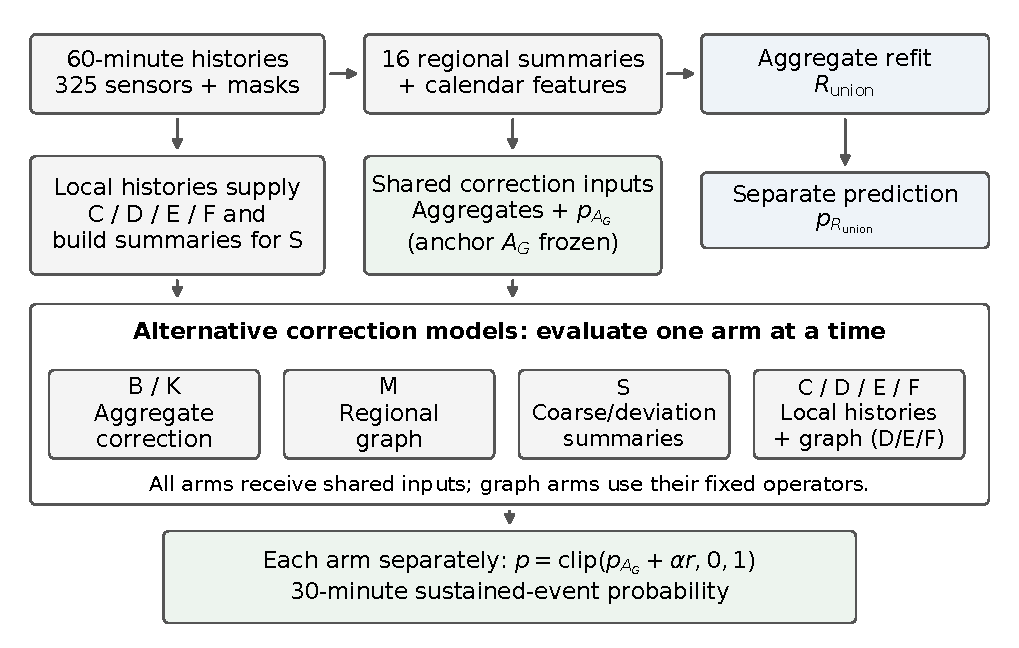
\includegraphics[width=\textwidth]{figures/overview.pdf}}
\caption{Alternative prediction paths, evaluated separately. $R_{\rm union}$ is an aggregate refit with its own output; all corrections use the frozen anchor $A_G$. B/K use aggregates, M adds regional messages, S adds graph summaries, and C/D/E/F use local histories. Initial summaries and S both require all-sensor ingestion.}
\label{fig:overview}
\end{figure}

\section{Predictors and Graph Representations}
\subsection{Frozen Anchor and Aggregate Controls}
The anchor $A_G$ is a GPU quantile-binned tree booster with 100 trees, at most 15 leaves, 64 candidate bins, minimum leaf size 20, and learning rate .1. Its L2 setting was selected from two choices within early training. $R_{\rm union}$ uses the same selected specification and feature transform, refitted on the exact union of the anchor and correction training examples at the same stride. Both have recoverable fitted weights and separate predictions; corrections remain anchored to $A_G$.

$A_{\rm mono}$ applies a positive-slope logistic map to the frozen anchor. It was fitted on out-of-sample anchor predictions in the correction period. B adds a compact aggregate-only residual learner, and K increases the aggregate parameter budget to approximately that of local and graph corrections. The main-study training selection chose B as the aggregate comparator and E as the expanded graph comparator. These choices remain fixed for test, even when another arm has a better observed score.

Every correction uses
\begin{equation}
 p_t=\operatorname{clip}_{[0,1]}\{p_{A_G,t}+\alpha r_\theta(I_t)\},
 \qquad r_\theta(I_t)=\tfrac12\tanh g_\theta(I_t).
\label{eq:correction}
\end{equation}
The residual head was initialized to zero and trained using ordinary all-time Brier loss plus $\lambda r_\theta^2$, with weight decay. Zero correction recovers the anchor exactly. This property does not guarantee better generalization after fitting. A global $\alpha\in\{0,\allowbreak .25,\allowbreak .5,1\}$ was selected in a separate training block. It scales the residual before clipping. The frozen final evaluation changes none of these values.

\subsection{Six Representations}
Table~\ref{tab:inputs} summarizes the arms. C applies a shared MLP to each ordered local history and a self-message branch before masked regional pooling. D replaces that self message with one normalized weighted neighbor average. The original operator is a row-normalized distance-similarity matrix. Its weights indicate proximity, not verified directed road flow. The row convention determines which source histories a receiving node averages, without identifying causal direction.

M first encodes the available regional summary histories and exchanges messages on the fixed regional operator $Q=RWL$. It receives no extra local measurements. S instead exposes a small collection of graph-dependent regional summaries at hop scales one, two, and four. E uses separate within-region and cross-region messages, concatenated with each node's own encoding. Its two neighbor streams share the same total available-neighbor denominator. They are not independently renormalized to equal strength. E\_internal sets the cross-region stream to zero while retaining that denominator and the same architecture.

F substitutes a sparse training-estimated dependency operator into D's message architecture. Sensor histories are first residualized against earlier-training calendar terms and regional common components. Absolute residual correlations define neighbors, with each row's nonself degree matched to D. The retained association is unsigned, so negative associations also become positive averaging weights. F does not preserve all indegrees, optimize adjacency jointly with the forecast loss, or reveal causal road directions. These distinctions limit interpretations of either success or failure.

\begin{table}[t]
\caption{Main inputs and processing. Every correction also receives the aggregate vector and frozen anchor probability. Parameter counts exclude the shared anchor.}
\label{tab:inputs}
\small
\begin{tabularx}{\textwidth}{l l >{\raggedright\arraybackslash}X r}
\toprule
Arm & Extra input & Representation & Parameters\\
\midrule
$A_G$, $R_{\rm union}$ & None & Aggregate tree predictors & Trees\\
$A_{\rm mono}$ & None & Monotone anchor map & 2\\
B & None & Aggregate correction & 38,209\\
K & None & Larger aggregate correction & 50,129\\
C & Full local histories & Shared temporal encoder, self message & 49,553\\
D & Full local histories & Distance-weighted sensor messages & 49,553\\
M & None & Messages among regional summaries & 49,937\\
S & \shortstack[l]{Local-derived\\summaries} & Coarse and deviation summaries at 1, 2, 4 hops & 50,321\\
E & Full local histories & Separate internal and boundary messages & 49,809\\
F & Full local histories & Frozen sparse dependency messages & 49,553\\
\bottomrule
\end{tabularx}
\end{table}

The message and temporal widths are 16, and the ordinary aggregate and final hidden widths are 32. K uses aggregate width 42. All local and graph outputs pass through the same regional interface where feasible. Differences remain in input dimension, number of channels, normalization and effective function class. A matched parameter count is a capacity control, not a proof of equal optimization difficulty. B versus C therefore compares fitted representations and learning problems; it does not isolate an intrinsic information value independent of the learner.

\subsection{Coarse State and Graph-Dependent Detail}
Let $L\in\mathbb{R}^{325\times16}$ lift a regional vector to sensors and let $R\in\mathbb{R}^{16\times325}$ average each nonempty region, so $RL=I$. For a fully observed vector $x$, write
\begin{equation}
 z=Rx,\quad u=x-Lz,\quad Q=RWL,\quad s_h=RW^hu.
\end{equation}
Then
\begin{equation}
 RWx=Qz+s_1,\qquad RW^hx=(RW^hL)z+s_h.
\label{eq:decomposition}
\end{equation}
S supplies the coarse and deviation terms separately at the fixed hop scales. Repeated sparse products compute these features without materializing dense powers. In general $RW^hL$ differs from $Q^h$, since omitted deviations can affect subsequent regional averages.

By established projection algebra, $s_1$ vanishes for every $x$ exactly when $RW(I-LR)=0$, or $RW=QR$. For directed operators, forward invariance $WL=LQ$ alone is insufficient; applicable symmetry or closure assumptions matter \cite{schaub}. These identities motivate S but do not establish sufficiency for the nonlinear event. The accompanying \path{reports/ONSET_GRAPH_STUDY_REPORT.md}, ``Multiscale construction and mathematical limits,'' gives the derivation and directed counterexample.

With missing inputs, S uses observed regional means and zero-filled unavailable deviations, equivalent to completing missing values by their observed regional mean (zero for an empty region). Equation~\ref{eq:decomposition} then describes this completed feature vector, not unknown speeds. Availability fractions accompany the features. The identity does not transfer to the mask-dependent neighbor normalization in D/E/F; missing future labels remain bounded, not imputed.

\subsection{Topology Controls and Attribution}
D's identity control is the matched C architecture. E has its own self-message and internal-only controls. Two outcome-blind rewiring seeds generate trained competitors for D and E through directed double-edge swaps. Each null preserves nonself edge count, per-node in/outdegree, source-row weight multisets and diagonal fallbacks. It changes neighbor identity, geometry and regional mixing. Cross-region edge count rises from 1,130 in the original graph to 2,228 in each null. Thus a real-versus-null difference is not a clean test of geometry while holding regional structure fixed.

The two fixed nulls are not uniform samples of the degree-constrained graph ensemble. They receive the same tuning allowance and all three training seeds. These are trained competitors, rather than post-training graph perturbations.

\section{Experimental Design}
\subsection{Chronology, Frozen Choices and Exposure}
The original split uses 108 complete training days through April 19, 36 validation days from April 20 to May 25, and 36 test days from May 26 to June 30. Incomplete March 12 is excluded from training. Input and outcome windows remain inside their split, with a two-sided 90-minute embargo at boundaries. Timestamps are naive in the release; a timezone convention is not asserted.

The main training pipeline separates six roles: anchor fitting through February 23; correction fitting from February 24 to March 16; early stopping from March 17 to 24; shrinkage and family selection from March 25 to April 1; calibration from April 2 to 9; and a final development gate from April 10 to 19. Windows crossing these boundaries are embargoed. All labels are observable before their role's cutoff. The anchor has 5,173 eligible fitting examples and the refit has 7,070. Correction training uses the later portion at stride three, matching its contribution to the refit's union. This addresses the older pilot's comparison between stride-12 early baseline training and denser later correction training.

Each correction family had two predeclared regularization choices, one tuning seed, and three retained seeds for the selected setting. AdamW used learning rate .001, weight decay .0001, batch size 256, at most 60 epochs and patience eight. Training minimized unweighted all-time Brier with residual regularization; selection used development onset Brier. No event weighting changed the probability estimand. Earlier rolling chronological evaluations are retained even when weak or unfavorable. Their overlaps and limited event counts prevent interpreting them as independent studies.

All validation days had been exposed during prior development. In an earlier pilot, onset was a favorable secondary endpoint. That observation motivated its registered primary role in the main graph comparison. The strengthened main comparison was less favorable to local information. We explicitly retain this history. It prevents retrospective relabeling of the earlier exploratory finding as a primary result.

The final test stage opened previously unexamined measurements only after the full protocol and verified implementation were committed. All required checkpoints were present. Their hashes, graph operators, transforms, shrinkage, calibration, thresholds and seed membership were fixed before access. No test outcome determined a fit, exclusion definition, threshold, representation or manuscript illustration. Test and validation are reported separately, without pooling their losses or event groups.

\subsection{Metrics, Uncertainty and Alarms}
Raw onset Brier is primary. Raw all-time Brier is secondary, and scores after frozen calibration are labeled separately. For each family we average the three seed-specific losses at each origin before temporal resampling. We do not average probabilities into an ensemble. Per-seed scores and their descriptive standard deviation remain available.

The registered raw onset comparison family is C minus B, D minus C, E minus D, and E minus B. Negative values favor the first arm. We use 2,000 paired calendar-block resamples with seed 20261007, three-day blocks as primary and one-day blocks as sensitivity. All origins in a selected day and their model/seed pairing remain together. Contiguous calendar segments are resampled separately, preserving gaps. Four-contrast Bonferroni percentile intervals use 98.75\% marginal coverage as an approximate familywise assessment. We also show pointwise 95\% intervals. These intervals condition on the fitted models and do not capture all training or development-selection uncertainty.

B versus $R_{\rm union}$ is a required secondary comparison. Graph-versus-aggregate and topology-control contrasts are descriptive, with pointwise intervals. F remains secondary regardless of its point rank. Practical scales carried forward from the protocol are a .0001 absolute and 1\% relative local benefit, or .00005 and .5\% graph benefit. Alarm tolerances are a recall loss of .02 or FPR increase of .01. These are pilot interpretation scales, not equivalence margins or a substitute for uncertainty.

Each predictor's positive-slope logistic calibrator was fitted on separate, out-of-sample training predictions. The calibration block contains only 30 onset-positive origins in five groups on four days. Strict alarms use $p>c$, where the frozen cutoff targets 5\% calibration FPR and excludes ties without jitter. The map is nondecreasing after endpoint clipping and cannot recover ranking among tied zeros. Test recall and FPR are measured, not assumed to inherit the calibration target.

Positive forecast groups merge origins separated by less than 30 minutes; a gap of at least 30 minutes starts a new group. A group is detected if any origin in it alarms. False-alarm groups use the same gap rule among alarmed non-event origins. These summaries account for repeated adjacent forecasts but do not turn groups into verified independent incidents. Event/non-event loss contributions, fixed-bin reliability and clipping diagnostics complement overall Brier.

\subsection{Computation and Verification}
All scientific numerics ran on one NVIDIA RTX 6000 Ada Generation GPU with PyTorch 2.8.0, CUDA 12.8 and driver 570.124.06. CPU work handled orchestration, file processing and rendering. Frozen raw and calibrated validation predictions replayed exactly before test access. The test replay also reproduced predictions exactly, with metric differences within the declared $10^{-12}$ tolerance. Checkpoint hashes, alignment checks, source revisions and detailed resource/replay records are preserved in \path{reports/FINAL_TEST_REPORT.md} and its linked artifacts. Existing timings are reused below.

\section{Results}
\subsection{Held-Out Support and Competitive Aggregate Controls}
The test has 10,333 timestamp-eligible origins, of which \TestEligible{} are scoreable. Six fail future coverage and none has disagreeing event bounds. There are 1,147 all-time positives. The onset population has \TestOnsetN{} origins and \TestPos{} positives, prevalence \TestPrevalence{}, grouped into 45 positive forecast groups on 25 days. Validation had 8,981 onset origins, 289 positives and 47 groups on 26 days. These differing populations are not combined.

\begin{table}[t]
\caption{Main-family Brier and frozen-threshold onset alarms. Correction entries average seed-specific scores, not probabilities. Validation is exposed development evidence; raw onset Brier is primary. Recall and FPR are test onset rates.}
\label{tab:scores}
\centering\small
\begin{tabular*}{\textwidth}{@{\extracolsep{\fill}}lrrrrrr}
\toprule
Model & \shortstack{Validation\\onset\\raw} & \shortstack{Test\\onset\\raw} & \shortstack{Test\\all-time\\raw} & \shortstack{Test\\onset\\calibrated} & Recall & FPR\\
\midrule
$A_G$ & 0.01411 & 0.01602 & 0.02060 & 0.01397 & 93.5\% & 4.87\% \\
$R_{\rm union}$ & 0.01217 & 0.01425 & 0.01852 & 0.01286 & 96.2\% & 5.29\% \\
$A_{\rm mono}$ & 0.01360 & 0.01467 & 0.01920 & 0.01381 & 93.5\% & 4.87\% \\
B & 0.01217 & 0.01521 & 0.01974 & 0.01399 & 92.8\% & 5.97\% \\
K & 0.01316 & 0.01535 & 0.01993 & 0.01412 & 93.2\% & 5.84\% \\
C & 0.01240 & 0.01537 & 0.01985 & 0.01406 & 93.2\% & 6.32\% \\
D & 0.01253 & 0.01515 & 0.01979 & 0.01399 & 92.8\% & 6.69\% \\
M & 0.01317 & 0.01512 & 0.01978 & 0.01381 & 92.4\% & 4.94\% \\
S & 0.01308 & 0.01524 & 0.01983 & 0.01386 & 92.8\% & 5.07\% \\
E & 0.01228 & 0.01504 & 0.01973 & 0.01399 & 92.8\% & 7.12\% \\
F & 0.01214 & 0.01538 & 0.01986 & 0.01418 & 92.7\% & 6.39\% \\

\bottomrule
\end{tabular*}
\end{table}

Aggregate refit $R_{\rm union}$ has the lowest raw onset and all-time point scores among the main families, \TestOnRUnion{} and \TestAllRUnion{} (Table~\ref{tab:scores}). Its frozen-calibrated scores are also lowest, \TestCalOnRUnion{} and \TestCalAllRUnion{}. Aggregate correction B has raw onset score \TestOnB{}. The secondary B minus $R_{\rm union}$ difference is .0009656, with three-day pointwise interval $[-.0000081,\allowbreak .0025347]$. This favorable refit point estimate remains uncertain and establishes neither superiority nor equivalence. The corresponding validation difference was near zero. The refit accesses the same union of fitting labels without adding local histories.

$A_{\rm mono}$ reaches raw onset \TestOnAMono{}, showing that a simple training-fitted probability map also competes with the residual arms. ``Raw'' denotes each arm's registered output before its additional final calibration map; $A_{\rm mono}$ is already a recalibration control.

\subsection{Registered Representation Contrasts}
Local-history correction C remains worse than aggregate correction B on test. Its onset difference is +.0001593, or a 1.05\% relative increase, with adjusted three-day interval $[.0000522,\allowbreak .0002315]$. This direction persists from the strengthened validation comparison and concerns this fitted local representation.

Distance graph D versus C changes direction from validation. Its test difference is -.0002203, a 1.43\% relative reduction. The pointwise interval $[-.0003640,\allowbreak -.0000063]$ favors D, but the adjusted three-day interval $[-.0004364,\allowbreak .0000268]$ crosses zero. Cross-region correction E versus D is -.0001074, a .71\% reduction, with adjusted interval $[-.0002318,\allowbreak .0000073]$. Its favorable validation point direction persists, but its adjusted exclusion of zero does not. E versus B reverses from an unfavorable validation point to -.0001684, or 1.11\%, on test; its adjusted interval $[-.0002960,\allowbreak .0000245]$ also crosses zero.

\begin{figure}[t]
\centering
\figalt{Four paired Brier contrasts are shown separately for exposed validation and frozen test, for onset and all-time outcomes. C minus B stays positive, while several graph contrasts change direction or remain uncertain.}{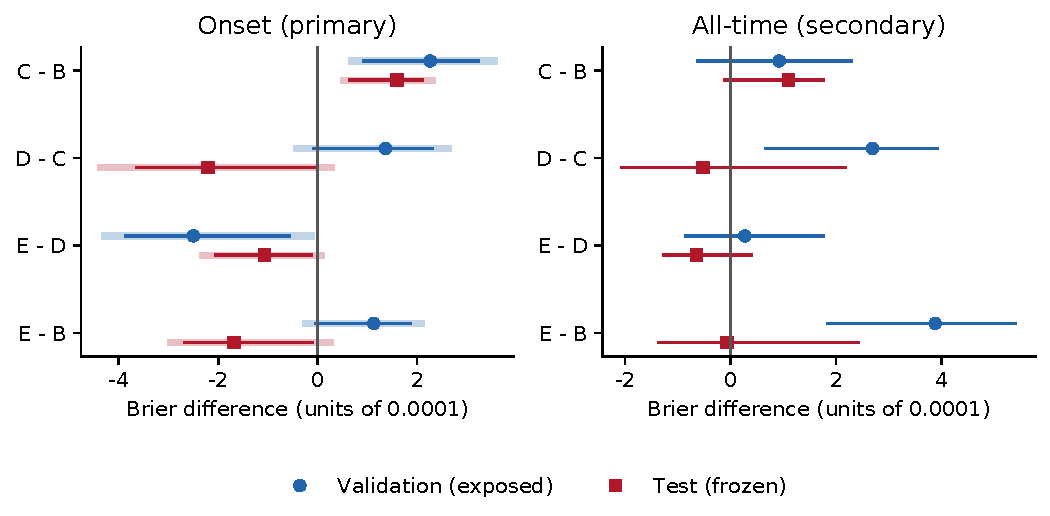
\includegraphics[width=\textwidth]{figures/effects.pdf}}
\caption{Paired effects for aggregate correction B, local histories C, distance graph D and cross-region correction E. Thin intervals are pointwise three-day 95\%; pale thick onset intervals are four-comparison adjusted. Left favors the first arm. Validation and test remain separate.}
\label{fig:effects}
\end{figure}

Graph point differences exceed the registered practical Brier scales, but uncertainty and alarms require separate assessment. One-day adjusted intervals favor D over C and E over B; the primary three-day intervals do not. This block-length sensitivity accompanies seed variation: E improves over B in two seeds and worsens in the third, while C is worse than B in all three. Seeds share the same event process and are not independent temporal replications.

All-time effects are generally smaller among corrections and do not follow every onset ordering (Fig.~\ref{fig:effects}). E's all-time score is \TestAllE{}, compared with B's \TestAllB{} and $R_{\rm union}$'s \TestAllRUnion{}. Dependency graph F, the best validation onset point estimate among corrections, scores \TestOnF{} on test and is worse than B in a secondary pointwise comparison. F remains secondary; it was never substituted for training-selected E.

\subsection{Topology and Regional Representation}
Cross-region correction E has the lowest raw onset point score among the six representations. Regional graph M scores \TestOnM{} and multiscale summaries S score \TestOnS{}. Their different inputs and processing paths yield small differences relative to temporal uncertainty.

D fails to beat both trained rewired controls. It is worse than rewiring seed 04 by .0000484, with pointwise interval $[.0000108,\allowbreak .0000854]$, while its comparison with seed 05 is uncertain. The particular distance topology therefore lacks consistent support in this architecture.

E beats both trained rewired controls on test by .0001886 and .0002492, with pointwise intervals $[-.0002705,\allowbreak -.0000692]$ and $[-.0004123,\allowbreak -.0000470]$. Both differences favor E in all three seeds. Its internal-only contrast is also favorable, while E versus E\_self remains uncertain. These secondary results were not consistently favorable on validation, and the nulls change regional mixing as well as neighbor identity.

\begin{figure}[t]
\centering
\figalt{Real versus trained null graph contrasts vary between validation and test. E beats both rewired controls on test, while D does not, and E versus its self control remains uncertain.}{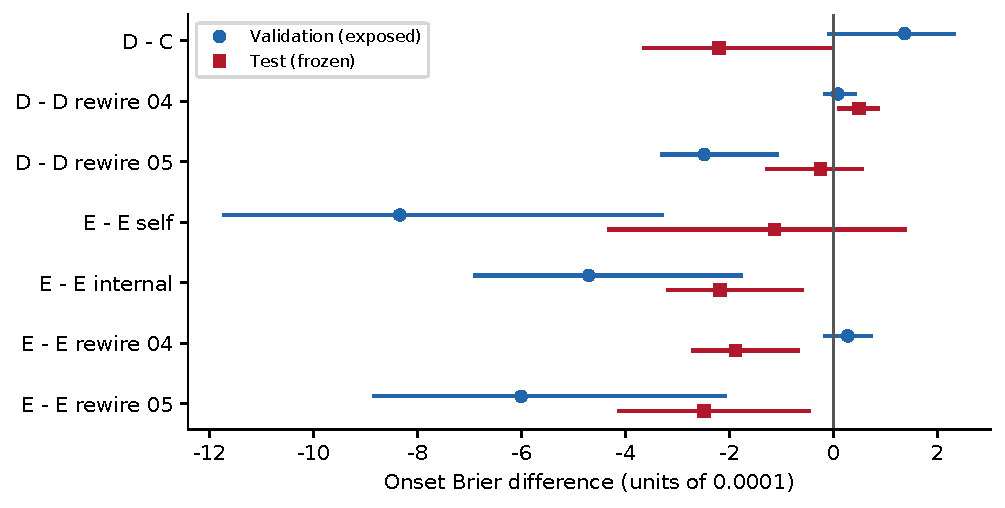
\includegraphics[width=\textwidth]{figures/topology.pdf}}
\caption{Distance graph D and cross-region correction E against trained topology controls, with pointwise three-day intervals. Nulls preserve degrees and row weights but change regional mixing. D--C also belongs to the primary family; the additional null/internal contrasts are descriptive secondary comparisons.}
\label{fig:topology}
\end{figure}

\subsection{Alarms, Calibration and Error Structure}
$R_{\rm union}$ achieves onset recall \TestRecallRUnion{} at FPR \TestFprRUnion{}. B, D and E share mean recall \TestRecallB{}, with FPR \TestFprB{}, \TestFprD{} and \TestFprE{}, respectively. E's FPR increase over B exceeds the registered one-percentage-point tolerance without a recall gain. Its favorable onset point Brier therefore does not yield an unqualified alarm improvement. $R_{\rm union}$ detects all 45 positive groups; B, C, D and E each detect an average of 43.33. Group detection is forgiving and should not be equated with every positive origin being detected.

\begin{figure}[t]
\centering
\figalt{Frozen test onset recall and false-alarm rates are plotted with three-day intervals. A second panel compares raw and frozen-calibrated reliability for aggregate refitting, aggregate correction and cross-region correction.}{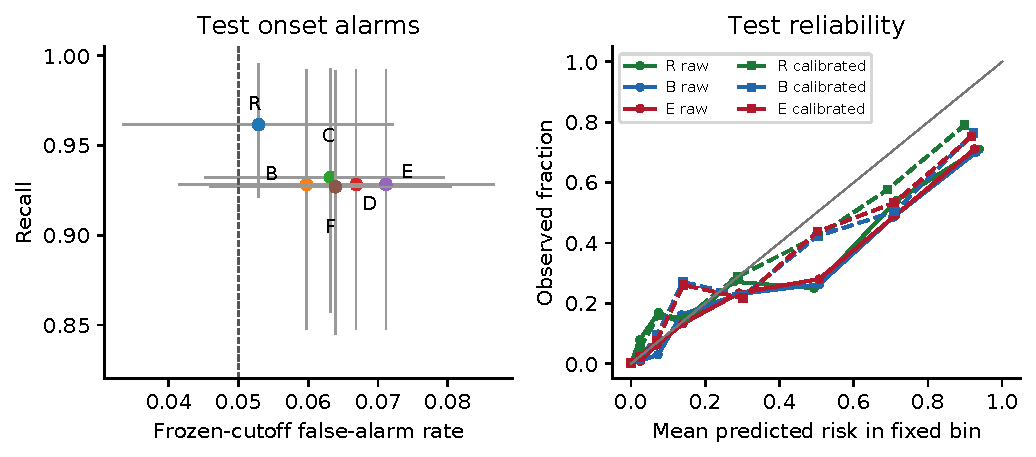
\includegraphics[width=\textwidth]{figures/alarms.pdf}}
\caption{Test alarm and calibration behavior. R denotes $R_{\rm union}$. The dashed vertical line is the training FPR target, not a test guarantee. Reliability bins pool seed-origin diagnostics without treating them as independent observations. Calibration does not select new thresholds.}
\label{fig:alarms}
\end{figure}

Frozen calibration improves test onset Brier for every main arm, reversing its adverse effect on validation. It leaves the observed alarm decisions unchanged here. $R_{\rm union}$'s calibrated onset score is \TestCalOnRUnion{}, compared with B \TestCalOnB{} and E \TestCalOnE{}. E no longer has a favorable calibrated point score relative to B. Calibration support is too limited to interpret this period-specific benefit as a general calibration guarantee.

Clipping remains substantial. B, C, D and E put approximately 86.6\%, 86.0\%, 85.8\% and 84.2\% of seed-origin onset predictions at exactly zero. M and S include a seed with a zero alarm cutoff. Monotone calibration cannot recover ranking within this tied mass, and no noise was added to resolve ties. These principal corrections overpredict mean onset prevalence, and high-probability bins overpredict observed risk (Fig.~\ref{fig:alarms}).

For B, event and non-event contributions to onset Brier are .00545 and .00976; for E they are .00560 and .00945. E reduces non-event loss but increases event loss, consistent with its unchanged recall. With $\delta=p-p_{A_G}$ after clipping, the evaluation verifies
\begin{equation}
 \overline{(Y-p_{A_G})^2-(Y-p)^2}
 =2\overline{\delta(Y-p_{A_G})}-\overline{\delta^2}.
\end{equation}
This established identity separates alignment with anchor errors from correction magnitude.

\subsection{Measured Costs}
Table~\ref{tab:cost} reuses the measured 128-origin validation workload: warm-cache history parsing, transfers, feature preparation, prediction and output transfer. Every correction includes the shared $A_G$ inference cost. Model restoration and graph preparation are separate setup costs; future-label creation is excluded. Means summarize three repeats for the first registered seed. Overlapping repeats provide no reliable latency advantage. Full repeats and fit times remain in \path{results/final_test/evaluate/historical_cost_summary.json} and the fitting records linked by \path{reports/FINAL_TEST_REPORT.md}.

\begin{table}[t]
\caption{Saved mean complete inference time for 128 origins, in seconds. Correction costs include the shared anchor. These small differences do not establish a speedup.}
\label{tab:cost}
\centering\small
\begin{tabular}{lr@{\hspace{2em}}lr}
\toprule
Aggregate arm & Mean seconds & Representation & Mean seconds\\
\midrule
$A_G$ & 0.2022 & C & 0.2087 \\
$R_{\rm union}$ & 0.2038 & D & 0.2080 \\
$A_{\rm mono}$ & 0.2074 & M & 0.2052 \\
B & 0.2066 & S & 0.2048 \\
K & 0.2061 & E & 0.2066 \\
 &  & F & 0.2068 \\

\bottomrule
\end{tabular}
\end{table}

Payload accounting specifies 4,632 float32 value bytes for the aggregate vector, 15,600 additional bytes for full local histories, or 2,304 for three regional deviation-summary streams, before masks, identities and graph metadata. These are representation sizes, not measured communication or memory savings. Both initial and graph summaries require all-sensor ingestion.

\section{Discussion and Limitations}
Competitive aggregate updating changes the interpretation of graph results. Aggregate refit $R_{\rm union}$ combines favorable point Brier and alarm behavior without local-history inputs. Its paired comparison with B remains uncertain, establishing neither superiority nor equivalence. Nevertheless, matching access to newer and more numerous labels is essential before attributing an advantage to sensor detail or graph processing.

Individual-history access and graph representation give different answers in this comparison. C loses to B on strengthened validation and frozen test, but its encoder, pooling and optimization define a particular learning problem. This fitted disadvantage does not imply zero intrinsic information in local measurements. Regional extrema and severe fractions may already capture useful detail; that is a possible explanation, not a sufficiency result. E's favorable secondary comparisons against both rewired controls coexist with uncertain primary graph contrasts and increased false alarms. They suggest a representation-specific effect worth distinguishing from a general graph benefit.

Three limitations constrain that interpretation. First, one dataset and a 36-day test period provide many overlapping origins but few event groups. Validation exposure influenced development, calibration had sparse support, and block intervals condition on fitted models rather than all training uncertainty. Second, the null graphs change regional mixing as well as neighbor identity, so E's secondary advantage cannot isolate road geometry. Third, F uses unsigned associations; its test disadvantage does not represent every learned-adjacency method. Neither exact projection identities nor computational replay establish forecasting sufficiency or numerical certification.

Measurement documentation remains incomplete. DCRNN documents public access and window generation \cite{release}, while Caltrans describes a registration-based archive and historical reprocessing \cite{caltrans}. The detector-to-HDF cleaning, smoothing, imputation and processing version are unresolved. Upstream processing could affect event support and apparent local dependence. The software license does not establish measurement-use or redistribution rights; missing documentation is distinct from an identified prohibition. Raw speeds are not redistributed. These provenance questions remain in the accompanying author-facing audit.

\section{Conclusion}
For this regional congestion-onset task, strong aggregate updating is competitive, the fitted local-history correction is unfavorable, and graph benefits depend on representation and assessment criterion. Cross-region messages beat two trained rewired controls in secondary test comparisons, yet favorable primary graph contrasts remain uncertain and false alarms increase. A common framework with matched label access, frozen chronological evaluation and explicit alarm criteria makes these distinctions visible. Useful probability estimates, meaningful topology effects and useful alarms require separate evidence.

\section*{AI Assistance}
An AI coding and writing assistant supported implementation, analysis orchestration, literature checking, manuscript drafting and editorial revision. No AI system is an author.

\bibliographystyle{splncs04}
\bibliography{references}
\appendix
\section{Per-Seed Onset Results}
\begin{table}[h]
\caption{All frozen test arms. Corrections retain seeds 20261001, 20261002 and 20261003 in order. Null suffixes 04/05 identify graph seeds 20261004/20261005. SD is descriptive with denominator three, not a confidence interval.}
\centering\small
\begin{tabular}{lrrrr}
\toprule
Arm & Seed 01 & Seed 02 & Seed 03 & SD\\
\midrule
$A_G$ & 0.016018 & -- & -- & 0.000000 \\
$R_{\rm union}$ & 0.014247 & -- & -- & 0.000000 \\
$A_{\rm mono}$ & 0.014674 & -- & -- & 0.000000 \\
B & 0.015521 & 0.015031 & 0.015085 & 0.000220 \\
K & 0.015741 & 0.015297 & 0.015027 & 0.000294 \\
C & 0.015715 & 0.015171 & 0.015229 & 0.000244 \\
D & 0.015312 & 0.014845 & 0.015296 & 0.000217 \\
M & 0.015341 & 0.014823 & 0.015185 & 0.000217 \\
S & 0.015423 & 0.014899 & 0.015387 & 0.000239 \\
E & 0.015057 & 0.014757 & 0.015317 & 0.000229 \\
F & 0.015668 & 0.014971 & 0.015494 & 0.000296 \\
E\_internal & 0.015683 & 0.014834 & 0.015271 & 0.000347 \\
D rew. 04 & 0.015222 & 0.014739 & 0.015348 & 0.000263 \\
D rew. 05 & 0.015480 & 0.014859 & 0.015191 & 0.000253 \\
E\_self & 0.015299 & 0.014832 & 0.015342 & 0.000231 \\
E rew. 04 & 0.015328 & 0.014803 & 0.015566 & 0.000319 \\
E rew. 05 & 0.015662 & 0.014769 & 0.015448 & 0.000381 \\

\bottomrule
\end{tabular}
\end{table}
\end{document}
